In this section we present our proposed system architecture and formulate the problem statement.

\begin{figure}
	\centering
	\usetikzlibrary{arrows}
\usetikzlibrary{automata}
\usetikzlibrary{positioning}
\usetikzlibrary{backgrounds}
\usetikzlibrary{fit}

\tikzset{
    state/.style={
           rectangle,
           rounded corners,
           draw=black, very thick,
           minimum height=0.6cm,
           minimum width=1cm,
           inner sep=3pt,
           text centered,
           node distance=0.9cm,
           },
    process/.style={
           rectangle,
           rounded corners,
           draw=black, very thick,
           minimum height=0.6cm,
           minimum width=1cm,
           inner sep=3pt,
           text centered,
           %node distance=1cm,
           },
    newprocess/.style={
           rectangle,
           rounded corners,
           draw=black, very thick,
           fill=lightgray,
           minimum height=0.6cm,
           minimum width=1cm,
           inner sep=3pt,
           text centered,
           %node distance=1cm,
           },
    processplaceholder/.style={
           minimum height=0.6cm,
           minimum width=1cm,
           %inner sep=3pt,
           text centered,
           %node distance=1cm,
           },
    closerstate/.style={
           rectangle,
           rounded corners,
           draw=black, very thick,
           minimum height=0.5cm,
           minimum width=5.32cm,
           inner sep=3pt,
           text centered,
           node distance=1cm,
           },
    abovish/.style={
           rectangle,
           rounded corners,
           draw=none,
           minimum width=1cm,
           text centered,
           node distance=1cm,
           },
    supercloserstate/.style={
           rectangle,
           draw=none,
           minimum height=0.2cm,
           minimum width=6.9cm,
           node distance=1cm,
           },
}

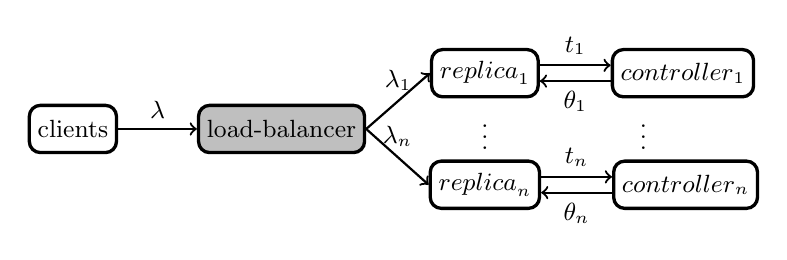
\begin{tikzpicture}[font=\small]
  \tikzstyle{surround} = [fill=black!20,very thick,draw=black,rounded
  corners, inner sep=5pt,] \tikzstyle{surroundblue} =
  [fill=blue!20,very thick,draw=black,rounded corners, inner sep=5pt,]
  \tikzstyle{surroundyellow} = [fill=yellow!20,very
  thick,draw=black,rounded corners, inner sep=5pt,]
  \tikzstyle{external} = [fill=none,very thick,draw=black,rounded
  corners, inner sep=15pt,]

% clients
\node[process] (clients){clients};

% load-balancer
\node[newprocess, right=1cm of clients] (lb){load-balancer};

% servers
\node[processplaceholder, right=1cm of lb] (replicaI) {$\vdots$};
\node[process, above=0cm of replicaI] (replica1) {$\text{replica}_1$};
\node[process, below=0cm of replicaI] (replicaN) {$\text{replica}_n$};

% controllers
\node[processplaceholder, right=1cm of replicaI] (controllerI) {$\vdots$};
\node[process, right=0.9cm of replica1] (controller1) {$\text{controller}_1$};
\node[process, right=0.9cm of replicaN] (controllerN) {$\text{controller}_n$};

% clients to lb
\draw[thick,->] (clients.east) -- (lb.west) node[midway, above] {$\lambda$};

% lb to replicas
\draw[thick,->] (lb.east) -- (replica1.west) node[midway, above] {$\lambda_1$};
\draw[thick,->] (lb.east) -- (replicaN.west) node[midway, above] {$\lambda_n$};

% replica to controllers
\draw[thick,->] ([yshift=+1mm]replica1.east) -- ([yshift=+1mm]controller1.west) node[midway, above] {$t_1$};
\draw[thick,<-] ([yshift=-1mm]replica1.east) -- ([yshift=-1mm]controller1.west) node[midway, below] {$\theta_1$};
\draw[thick,->] ([yshift=+1mm]replicaN.east) -- ([yshift=+1mm]controllerN.west) node[midway, above] {$t_n$};
\draw[thick,<-] ([yshift=-1mm]replicaN.east) -- ([yshift=-1mm]controllerN.west) node[midway, below] {$\theta_n$};

\end{tikzpicture}

	\caption{Architecture of a brownout application featuring multiple replica}
	\label{fig:architecture}
\end{figure}

Figure~\ref{fig:architecture} presents the architecture of a brownout-compliant application featuring multiple replicas, which reflects established practices in cloud applications~\cite{Barroso09}. The main processes are the clients, which are the users of the cloud application, the load-balancer which directs loads towards replicas, the replicas themselves, implementing application logic, and the controllers, which decides the amount of optional content that each replica should serve. Let us describe each process and highlight its specificities related to brownout-compliance.

Clients send requests at a constant rate $\lambda$ which are send to the load-balancer. The load-balancer forwards these requests to one of the $n$ replicas. As a results, each replica $i$ receives requests with a rate $\lambda_i = w_i \cdot \lambda$, such that $\sum_{i=\overline{1,n}} w_i = 1$, where $w_i$ represents weights computed by the load-balancer.

A replica $i$ may respond to each request in two modes: partially, where only mandatory content is included in the reply, or fully, where only mandatory and optional content is included. The service times for partial and full replies is $\mu_i$ and $M_i$, respectively. Obviously, partial replies are faster to compute than full ones, since the optional content does not need to be computed, hence, $\mu_i>M_i$. Whether the replica serves requests partially or fully depends on a parameter $\theta_i \in [0, 1]$, which represents the probability of serving optional content. Assuming the replica is not saturated, it serves requests fully at a rate $\lambda_i \cdot \theta_i$ and partially at a rate $\lambda_i \cdot (1-\theta_i)$. To aid load-balancing decisions, each replica piggy-bags the current value of $\theta_i$ through the reply, so that this value can be observed by the load-balancer.

The parameters $\theta_i$ are computed by controllers based on a parameter $\tau$, the target average response-time. Each replica $i$ periodically reports the average observed response-time $t_i$ to its controller. In exchange, the controller computes a new value $\theta_i$ to close the feedback loop and maintain average response-time.

Given the above architecture, the brownout load-balancing problem can be stated as follows. Assuming the load-balancer can measure $\lambda$, $t_i$ and $\theta_i$, compute the values $w_i$ that maximize $\sum_{i=\overline{1,n}} \lambda w_i \theta_i$.

